\section{Kalibrierung der Brille}

Wie kalibriert man eine Durchsichtbrille in einem Auto?

\subsection{Workflow}
    Um eine 3D-Durchsichtbrille so zu kalibrieren, dass auf dieser reale und authentisch wirkende 3D Welten angezeigt werden können, muss präzise kalibriert sein. Wichtig ist dies nur für die prezise Simulation einer AR-Welt. Dies wird wichtig um die Durchsichtbrille für diverse Dinge im UUmfang der kognitiven Automibile zu verwenden. Hierzuu gehören Anwendungen, bei den z.B. Fußgänger SImuliert werden um menschliche Fahrerinteraktionen zu messen und als Lerndaten zu aquireren. Eine weitere Anwendung wäre die SImulation von simulierten Daten des Fahrzeuges für den Fahrer, damit dieser in einer Simulierten Welt beurteilen kann, wie gut das kognitive Automobil sich einer Sitziuation, z.B. dem Einparken verhält. Ebenfalls wird es möglich, mit einer Kalibrierten Brille simulierte neue Bedienelemente eines Autos zu testen und deren Wirkung auf den Fahrer auszuprobieren.

    Hierzu werden die Parameter benötigt, mit denen die Bilder für ein solch akkurates stereoscopic 3D benötigt werden. Zu diesen Parametern zählt die Position der Augen, die Position der Bildschirme in den Brillengläßern und die Öffnungswinkel, mit denen ein einzelnen Individuum durch eine spezifische Brille sehen kann.

    Um diese Parameter zu Bestimmen haben wir uns auf ein interaktives Kalibrierungsverfahren geeinigt, da es wichtig ist, dass die Kalibrierung komfortabel und ohene große Hilfestellung von statten geht, da es für jeden Benutzter nötig ist, die Brille individuell zu kalibrieren. Das Minimum an benötigten Punkten um die Position eines Auges zu bestimmen sind zwei Geraden, also zwei Punkte auf einer Sichtiline je Geraden. Um die Daten präziser zu machen können mehrere Geraden verwendet werden, die dann einen Genaueren Schnittpunkt ermöglichen, es sollen aber immer nur 2 Punkte je Gerade verwendet werden, da das aufeinanderlegen von 3 Punkten in unangenhemen Positionen für den Benutzer während der Kalibrierung endet.

    Der erste Ansstz war es einen Punkt im Auto zu verwenden, der in seiner Position bekannt ist und durhc Bildverarbeitung erkannt werden kann und n Punkte auf der Brille. Hierbei hat sich jedoch herausgestellt, dass der Abstand der einzelnen Schnittlinien in einem sehr kleinen WInkel von statten geht und somit fehleranfällig ist. Der zweite Ansatz verwendet den Bildschirm, der im Auto verbaut ist und die Brillengläser. Hiermit sind beidseitig die Punkte variabel und können somit so gewählt werden, dass sich Messfehler nicht so gravierend auswirken wie im vorherigen Ansatz. Desweiter ist das Verfahren erweiterbar auf eine Onlinebewertung während der Kalibrieung, so dass über ein Algorithmus passende Punkte ausgewählt werden können, um die Kalibrierung zu optimieren.

    Im Ablauf werden nun also Punkte auf dem Brillenglas angezeigt, die der Benutzer per Klick auf die Stelle auf dem Bildschirm markiert, so dass sie für ihn übereinander liegen. Somit konnte ein idealer Kompromiss zwiscen Benutzerfreundlichkeit und der Aquisition von geeigneten Linienpaaren gefunden werden.


\subsection{Bestimmung von Punktepaaren}
\subsubsection{Konzept}
Um nun also Punktepaare für die Kalibrieung aufzeichnen zu können, ist die Grafikausgabe der Software nötig. Hierzu wurden zwei Anwendungen als ROS Nodes implementiert. Die Nodes werden mittels der Frameworks SDL und Qt umgesetzt.
\subsubsection{Anzeige auf der Brille}
Eine Vollbildanzeige mit fester Auflösung der nativen Auflösung der Brillenanzeige wird mittels SDL implementiert. Diese Anwendung erkennt automatisch die Brille als zweiten Bildschirm und wählt diesen für die Anzeige aus. Ansonsten ermöglicht die Anwendung es, einen Punkt an eine per ROS-Paket vorgegebenen Position anzuzeiegn.
Screenshot
\subsubsection{Anzeige auf dem Bildschirm}
Ein Fensteranwendung implementiert mit Qt zeigt die für die Bildverarbeitung nötigen marker (siehe Kapitel??) an und nimmt die Klickpositionen vom Nutzer entgegen. Die ermittelte Clickposition wird als ROS-Paket versendet.
Screenshot!


\subsection{Koordinatentransformation}
\subsubsection{Übersicht}
Die Koordinatentransformationen sind nötig, um aus den Punktepaaren (wie in Kap. ?? beschrieben) , Koordinaten im 3D Weltkoordinatensystem zu erhalten. Nur aus Punkten in einem einheitlichen Koordinatensystem können später korrekte Gerade berechnet werden.
Die Eingaben für das Verfahren erhält die Anwendung aus ROS-Paketen, siehe hierzu in Kapitel ??.
\subsubsection{Weltkoordinatensystem}
Das Weltkoordinatensystem für die Transformation hat seinen Ursprung in der Camera, gerichtet in Scihtrichtung mit der Knvention angelehnt an Kamerasysteme: x nach rechts  ,y nach unten, z nach vorne.
\subsubsection{Transformation für Brillenpunkte}
Das ausgewählte Koordinatensystem macht es einfach die Transformation von einem Brillenpixel in das Weltkoordnitensystem abzubilden. Es handelt sich um eine statische Transformation, da die Camera fest mit der Brille verschraubt ist. Die Herausforderung besteht darin, den virtuellen Bildschirm der Brille abzubilden. In den einzelnen Brillengläsern befindet sich Optik (Lines und ein Spiegel), mit denen dem Brillenträger ein großer Bildschirm Simuliert wird. Da es für uns jedoch nicht möglich war, festzustellen, ob für jeden Brillenträger die Anzeige gleich war, haben wir folgenden Verfahren angewendet: Wir haben den virtuellen Bildschirm, projeziert per strahlensatz, auf einen weiteren virtuellen Bildschirm genau im Mittelpunkt der Brille festgelegt. Dieser Bildschirm ist unabhängig vom Benutzer, da zu Vermessung dieses Bildschirmes der Abstand zum virtuellen Bildschirm keine Rolle spielt.
Die Wahl des virtuellen Bildschirms genau in der Brillenmitte hat ebenfalls den Vorteil, dass die gewonnenen Daten später auch für die Berechnung des Öffnungswinkels verwendet werden können, da diese identisch mit den physikalischen Brillengläsern sind.
Die Position des Bildschrimes wurd aus empirischen Ergebnissen gewonnen. Hierzu haben wir die Brille wagerecht zu einer Wand festgeschraubt und Punktepaare zu einem von Hand vermessenen Auge aufgenommen. Hierzu haben wir Punktekoordinaten auf dem Bildschirm zu konstanten Punkten auf der waagerecht zur Brille montierten Referenzwand (mit Punkten) vermessen. Die Brille wurde in die für den jeweiligen Probanden korrekte Position gebracht, so dass es genau für einen Öffnungswinkel die Referenzwand füllend im Bild sehen kann. Anschließend wird der Abstand zur Wand vermessen. Aus dem Abstand zur Wand und den Vermessenen Punkten auf der Wand, konnte mit Hilfe der gemessenen Pixel auf der Brille, die größe eines Pixel auf unserem virtuellen Bildschirm innerhalb der Brille erechnet werden. Der Abstand auf dem referenzbildschirm war für jeden Probanden gleich, die angeklickte Position war ebenfalls gleich, jedoch der Abstand zur Wand leicht verschieden, da verschiedene Probanden einen leicht Abweichenden Sichtöffnungswinkel hatten, da die Augen je nach physiologischen Eigenschaften verschieden weit hinter der Brille sich befinden. Hierdurch war es uns möglich eine Fehlerrechnung über alle Daten durchzuführen, da wir 15 Punkteppare hatten. Hierdurch kamen wir zu relativ genauen Ergebnissen des Brillenbildschirms:
    
    Statisch ermittelte Werte:
    Pixelgröße (links und rechts):      2.5219887302047E-02 cm/px 
    Größe des virtuellen Bildschirms (links und rechts):      1
    Position des Bildschirms (links):
    Position des Bildschirms (rechts):
        
Durch diese Ausmessungen konnte die  Transformation eines Koordinatenpunktes u,v in Weltkoordinaten auf zwei einfache Transformationen vereinfacht werden

    1. Statische Transformation: Translation vom Oberen linken virtuellen Bildschirmpixel zum Ursprung

    2. Dynamische Transformation: Translation um u,v Pixel nach obiger Vermessung umgerechnet in Meter

In der Implementierung wurde noch folgende Vereinfachung festgestellt: Da die virtuellen bildschirme immer eine parallele Ebene zur x,y-Achsen-Ebene aufstellen, kann die transformation durch eine einfache Addition durchgeführt werden

    Listing einfügen.

\subsubsection{Transformationen für Bildschirmpunkte}
Die Transformation von einem Bildschirmpixel in das Weltkoordinatensystem stellt andere Herausforderungen. Der Bildschirm kann als eine physikalische Gröse angesehen werden und vermessen werden. Es liegen konstante DPI-Werte vor, es kann also ebenfalls eine statische Transformation von einem Referenzpunkt auf dem Bildschirm zum angeziegten Punkt geschehen. Hierzu ist lediglich eine Transformation nötig, die die DPI-Werte des Bildschirms berücksichtigt und durchführt. Der Referenzpunkt des Bildschirms haben wir innerhalb unserer Anwendung (sihe Kapitel ??) gewählt, da dieser somit invariant gegen verschiebungen bleibt. Bei diesem Vorgehen besteht jedoch die größte Herausforderung darin, dass die Position des Bildschirmes benötigt wird. Heirzu wird die Camera mit Bildverarbeitung eingesetzt. Der erste Ansatz war es, openCV mit einem Schachbrett zur Erkennung zu verwenden. Da sich während der Implementierung herausgestellt hat, dass einiger Code, der beim Einsatz von openCV nötig ist, durch die Bibiolothek ALVAR, die sich ebenfalls noch wesentlich einfacher in ROS integrieren lässt abnimmt, wurde die Strategie geändert. Drei ALVAR Marker werden nun mittels der Webcam erkannt und zur Entfernungsbestimmung vermittelt. Hiermit sind nun beide Transformatione auch für die Berechnung der Position vorhanden. Dieser Ansatz bietet den Nachteil, dass ALVAR eine gewisse ungenauigkeit und eine gewisse Verzögerung mit sich bringt, wodurch die Benutzbarkeit erschwert wird. Ein längerfristiges Ziel sollte es also sein, die Integration des Headtrackingalgorithmuses auch in die Kalibrieung einzufügen.
    Statisch ermittelte Werte:
    Pixelgröße:
    Größe eines Markern in Pixeln/CM:
Das Konkrete Vorgehen beschreibt sich bezüglich der Transformation folgendermaßen:

    1. Dynamische Transformation:  Translation  um u,v der auf der Fensterfläche angeklickt wurde auf den Referenzpunkt der Anwendung (konkret, dem Mittelpunkt des obigen linken Markers) 

    2. Dynamische Transformation: Translation um die von ALVAR bestimmte entfernung

Um auf den Referenzpunkt zu gelangen, gibt es eine triviale Addtion, um den statischen Offset der Anzeigelemente und der centrierten ALVAR position zu kompensieren. Um nun die Translation um einen u,v Pixel zu realisiren, wird eine Ebene durch die drei marker gelegt und daruf die Verschiebung durchgeführt. Im Anschlass kann die Rücktransformation zum Koordinatenursprung geschehen.

    Listing einfügen



\subsection{Stereoskopisches 3D}

\subsubsection{Allgemeine Information}
Es existieren mehrere Gründe des menschliches Raumwahrnehmung.
Menschen sehen die Objekte dreidimensional wegen der Linearperspektive, relativer Größe zur anderen Objekte, Verdeckung der Objekten und wegen stereoskopisches Sehen. 
Stereoskopisches Sehen vermittelt durch die beidäugige Betrachtung von Objekten und Gegenständen eine echte, messbare Tiefenwahrnehmung und räumliche Wirkung des Außenraums. 
Das passiert mit der Hilfe beider unseren Augen.
Jede Auge bekommt ein eigenes Bild und sendet das ins Gehirn. 
Dort werden diese beide Bilder zu eine einzige zusammengefasst.
Genauere Beschreibung ist im Abb. \ref{fig:3D} zu finden.

\begin{figure}[h]
   \centering
   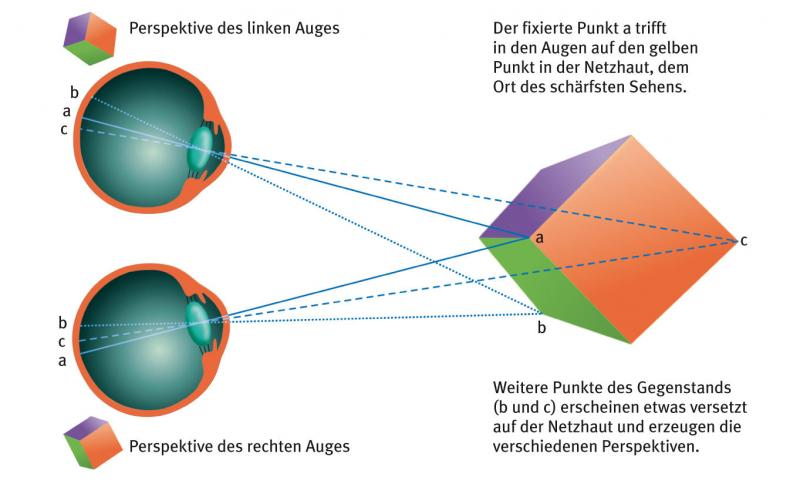
\includegraphics[width=0.45\textwidth]{3D-bild}
   \caption{steteoskopisches Sehen}
   \label{fig:3D}
\end{figure}

Die Bilder des linken und rechten Auges sich an manchen Stellen unterscheiden und menschliches Gehirn kann aus dieser Unterschiede die Positionen, Formen und Großen der Objekte extrahieren.

Damit ein Bild dreidimensional aussieht, ist meistens genug mit ungefähren Werten zu arbeiten.
Man nimmt zwei unterschiedliche Bilder, die anhand der mittlere Werte ausgerechnet werden, und zeigt jeder Auge eine davon. 
Damit bekommt man ein 3D-Bild. 
Für manche Anwendungen (wie 3D-Filme, oder sterioskopische Bilder) ist schon genug,  dass ein Bild als 3D interpretiert wird. 
Für uns aber nicht, da mit so eine Realisation unterschiedliche Menschen sehen dasselbe Bild unterschiedlich.
Alle Menschen werden diese Bilder als 3D interpretieren, aber die Position und Größe der gesehenen Objekte kann sich stark unterscheiden.
Für die Anwendungen, wie Testen des autonomes Fahrens des Fahrzeugs, sind aber diese Werte entscheidend.
Es ist sehr wichtig, ob ein anderes Fahrzeug schon getroffen ist, oder nicht.
Um die benötigte Genauigkeit zu realisieren, sind gemittelte Werte nicht genug.
Eine individuelle Kalibrierung der Brille soll diese Genauigkeit ermöglichen.

\subsubsection{Geometrische Beschreibung der Kalibrierung}
Dieses Kapitel beschreibt wofür die Kalibrierung durchgeführt wird und welche Daten dafür benötigt werden.
Die gegebene Daten sind im Abb. \ref{fig:geom} dargestellt. 

\begin{figure}[h]
   \centering
   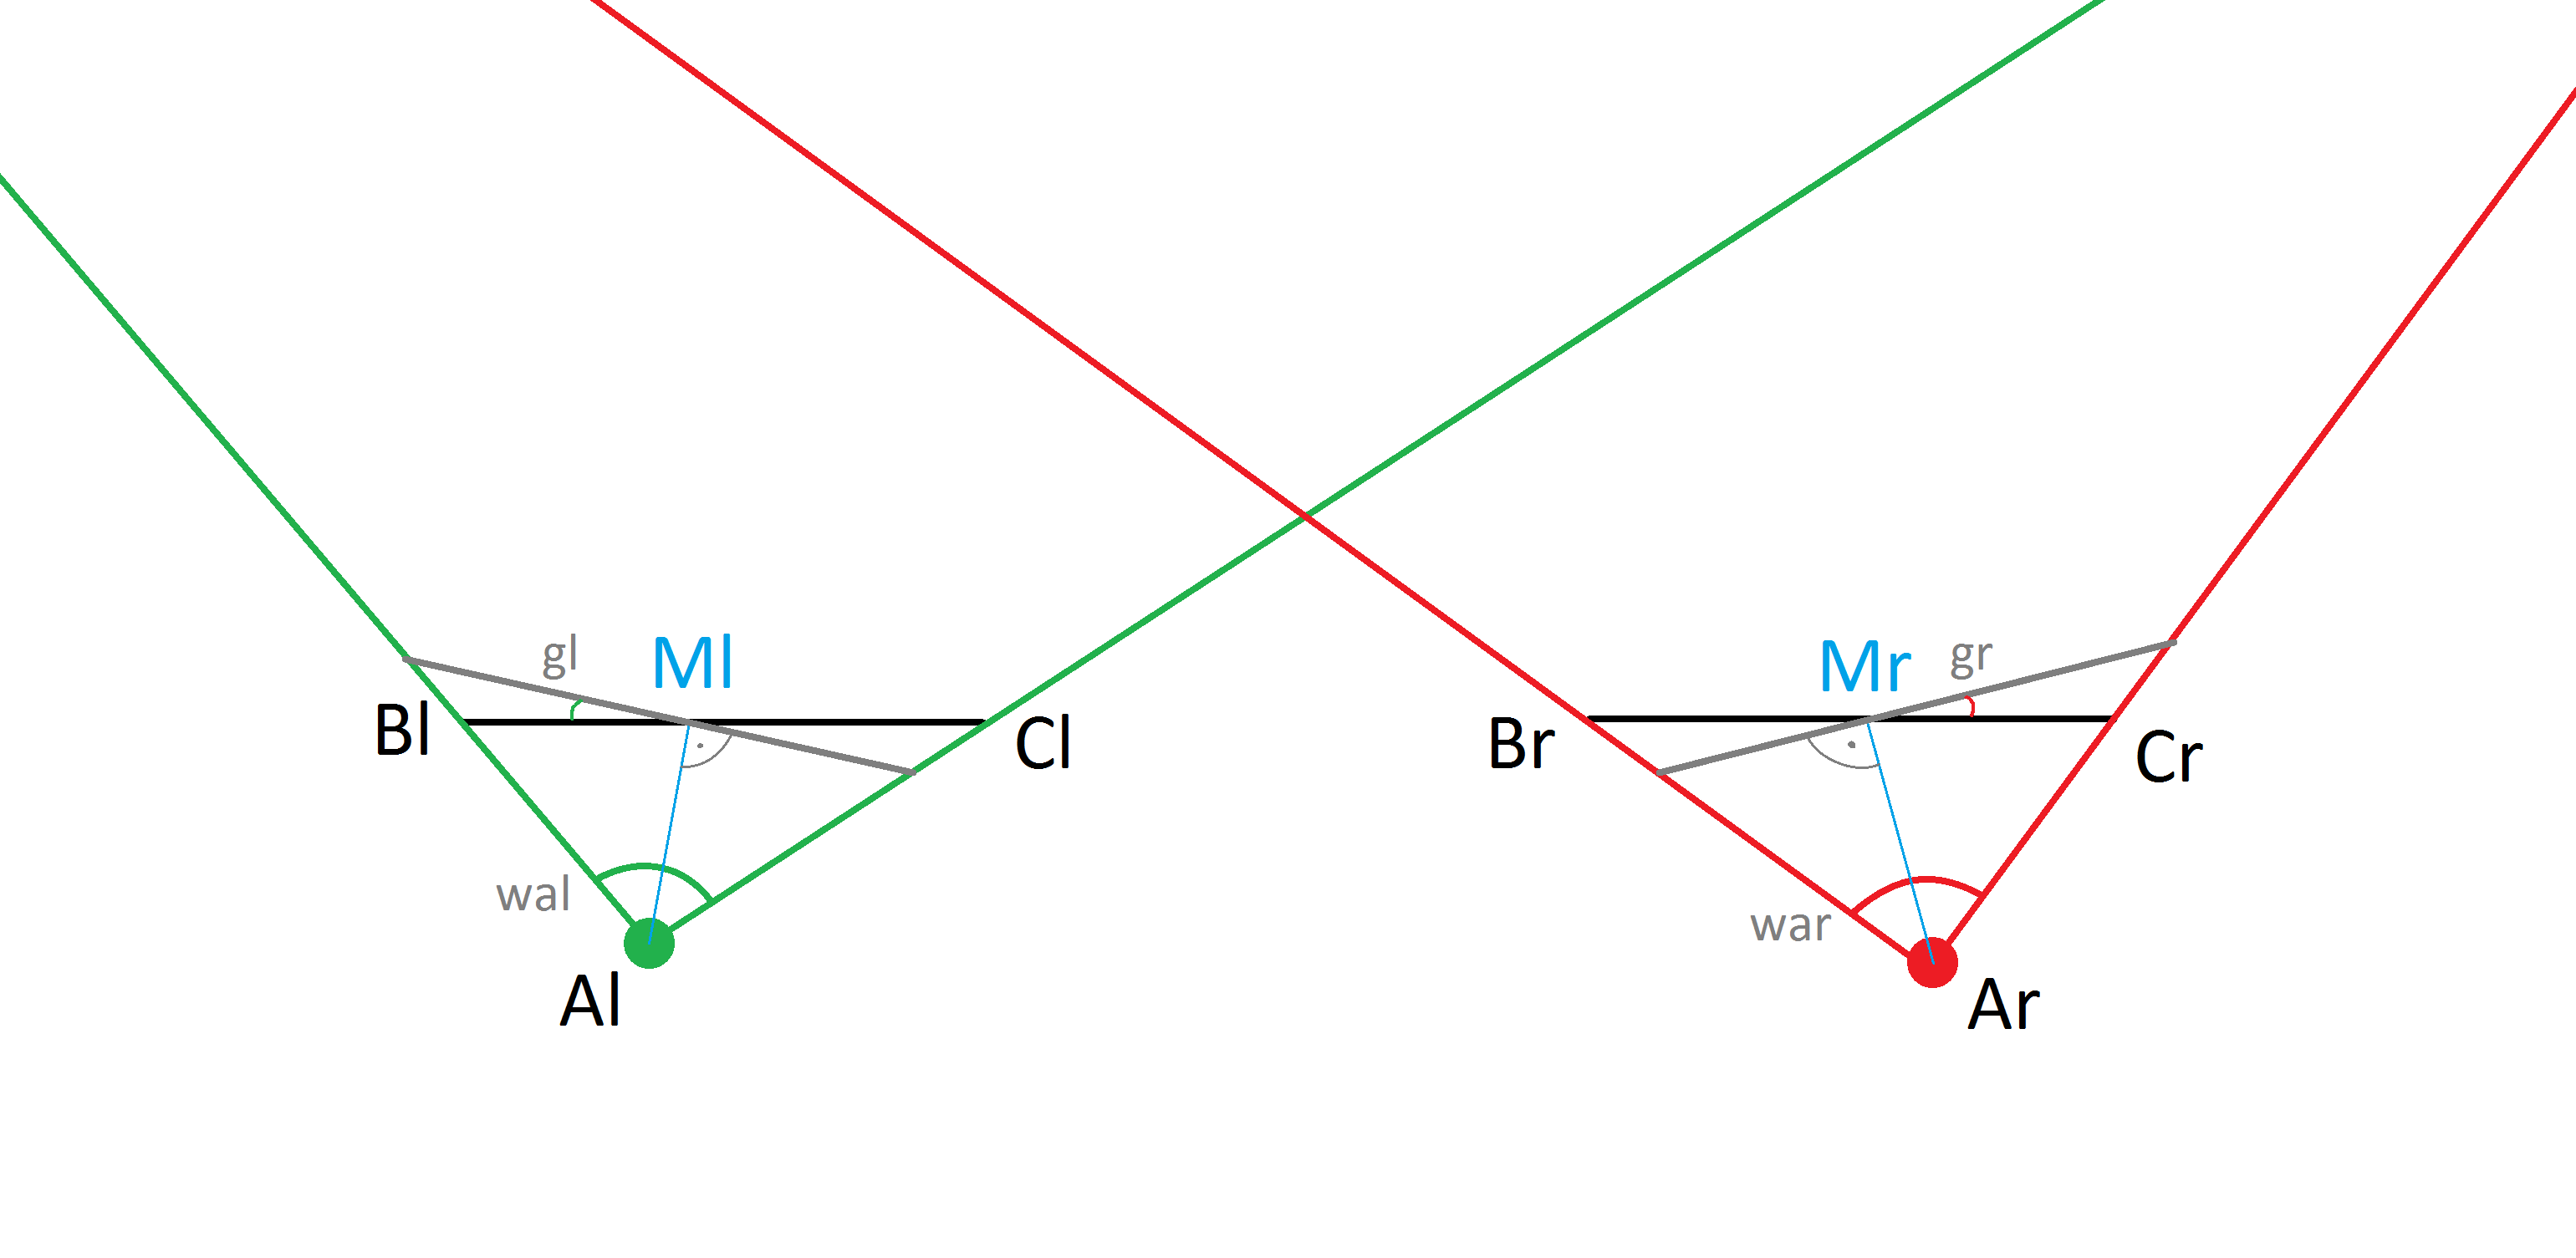
\includegraphics[width=0.45\textwidth]{kalibr-geometrie}
   \caption{Geometrische Beschreibung der Kalibrierung}
   \label{fig:geom}
\end{figure}

Punkte Bl, Cl bzw. Br, Cr sind die Endpunkte des linkes bzw. rechtes Bildschirms der Brille.
Die Punkte Al (grün) bzw. Ar (rot) beschreiben die Positionen der Augen.
wal bzw. war sind die Sehwinkel des Benutzers durch welche die Bildschirme und dort dargestellte Objekte gesehen werden. 
Blaue Linien ml und mr sind Winkelhalbierenden.

Für die Anzeige der Bilder auf der Brillenbildschirme, werden Augen als Kameras interpretiert und damit werden benötigte Bilder erstellt.
Dementsprechend sind die Winkeln wal und war die Öffnungswinkel dieser Kameras.
Wie auf dieser Abb. ref{fig:geom} gut zu sehen ist, müssen die Augepositionen nicht unbedingt in der mitte des Bildschirms liegen.
In meisten Anwendungen, die Kameras simulieren, ist aber vorausgesetzt, dass die Kameras in der Mitte sind.
Das ist das selbe, wie Winkelhalbierende der Öffnungswinkel senkrecht zur Bildschirm ist.
Wir nehmen an, dass dafür benötigte Drehwinkel gl bzw. gr spielt keine entscheidende Rolle in der Bildanzeige.
Mit dieser Annahme rechnen wir die Winkeln gl und gr aus  um die Virtuelle Bildschirme theoretisch zu drehen.
Das wird benötigt um passende Daten für die Benutzung anderer Anwendungen zu bekommen.



